\chapter{Sztuczne sieci neuronowe}
W~uczeniu maszynowym poprzez \textbf{sztuczne sieci neuronowe} rozumiana jest rodzina statystycznych modeli
uczenia się zainspirowanych biologicznymi sieciami neuronowymi. Mechanizmy te~są wykorzystywane do~estymacji
lub~aproksymacji funkcji, które zależą od~wielu wartości wejściowych i~są co~do~zasady nieznane.

Sieć neuronowa składa się~z~wielu połączonych ze~sobą jednostek (zwanych neuronami), które wymieniają między
sobą informacje. Połączenia między neuronami posiadają przypisane wagi, które w~trakcie uczenia sieci
są~modyfikowane. Typowo każdy neuron na~wejściu otrzymuje zbiór wartości (pochodzący z~wyjść innych neuronów
lub~będący danymi wejściowymi sieci). Następnie wartość każdego z~wejść jest mnożona przez~wagę przypisaną
do~odpowiedniego wejścia. Tak otrzymana suma jest poddawana działaniu funkcji aktywacji, która jest
charakterystyczna dla~danego typu neuronu i~nie~ulega zmianie wraz z~działaniem sieci.

\section{Model neuronu}
Przykładowym neuronem używanym powszechnie w~sieciach neuronowych jest neuron z~sigmoidalną funkcją aktywacji
(nazywany również neuronem sigmoidalnym). Schemat takiej jednostki przedstawiono na~poniższym rysunku
(rys.~\ref{img:model-neuronu}).

\begin{figure}[H]
	\centering
	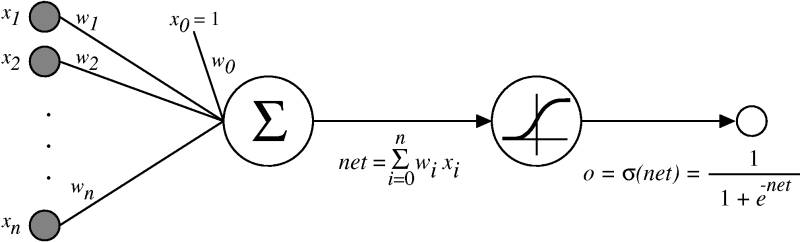
\includegraphics[width=\linewidth]{img/sigmoid-neuron.png}
	\caption{Model neuronu}
	\label{img:model-neuronu}
\end{figure}

W~pierwszej fazie działania neuronu sumowane są wartości na~wejściach neuronu pomnożone przez~odpowiadające
im~wagi. W~drugiej fazie dla~otrzymanej sumy obliczana jest wartość funkcji sigmoidalnej
$f(x)=\frac{1}{1+e^{-x}}$, która stanowi wartość wyjściową neuronu.

Innym często stosowanym neuronem jest neuron o progowej funkcji aktywacji, tzn.~dla~wartości powyżej pewnego
progu przyjmuje wartość 1, a~dla~pozostałych wartości przyjmuje 0 (lub -1). Wyjścia jednostek tego typu
zazwyczaj są~jednocześnie wyjściami całej sieci neuronowej i~nie~są przesyłane na~wejścia innych neuronów.

\subsection{Funkcje aktywacji}
W~neuronach wykorzystywane są bardzo różne funkcje aktywacji (\cite{activation-functions}). Każda z~nich zawiera swoje
zalety i~wady. W~niniejszej podsekcji przedstawiono i~omówiono wybrane funkcje.

\subsubsection{Funkcja liniowa}
Najprostsza z~możliwych funkcji aktywacji. Dokonuje liniowego przekształcenia na~wartości wejściowej
(rys.~\ref{rys:f-liniowa}). Jest rzadko stosowana do~zadań klasyfikacji w~sieciach neuronowych, gdyż~sieć składająca
się~z~neuronów o~liniowej~funkcji aktywacji nie~może modelować nieliniowych funkcji.

\begin{minipage}[t]{\textwidth}
\begin{equation}
f(x)=x
\end{equation}
\begin{figure}[H]
    \centering
    \begin{tikzpicture}
        \begin{axis}[
            scale only axis, % The height and width argument only apply to the actual axis
            height=5cm,
            width=0.9\textwidth,
            xtick={-1,1},
            axis x line=center, axis y line=center,
            xlabel=$x$,
            ylabel=$f(x)$
            ]
            \addplot [
                domain=-1.1:1.1,
                color=red
            ]{x};
        \end{axis}
    \end{tikzpicture}
    \caption{Funkcja liniowa}
    \label{rys:f-liniowa}

\end{figure}
\end{minipage}

\subsubsection{Funkcja progowa}
Funkcja nieliniowa, a~więc nadająca się~do~zadań klasyfikacji. Posiada jednak wadę przeszkadzającą w~uczeniu sieci
z~wykorzystaniem metod gradientowych: nie~ma~ciągłej pierwszej pochodniej. Funkcja została przedstawiona na~rysunku
\ref{rys:f.progowa}.

\begin{minipage}[t]{\textwidth}
\begin{equation}
	f(x) =
	\begin{cases}
	0 & x<0, \\
	1 & \textrm{w p.p.}
	\end{cases}
\end{equation}

\begin{figure}[H]
    \centering
    \begin{tikzpicture}
        \begin{axis}[
            scale only axis, % The height and width argument only apply to the actual axis
            height=5cm,
            width=0.9\textwidth,
            xmin=-3,xmax=3,
            ymin=-0.5,ymax=1.5,
            axis x line=center,
            axis y line=center,
            xtick={-3,3},
            ytick={-0.25, 0 , 0.5, 1},
            xlabel=$x$,
            ylabel=$f(x)$]
            \addplot[red, samples=1000] {(x>=0)};
        \end{axis}
    \end{tikzpicture}
    \caption{Funkcja progowa}
    \label{rys:f.progowa}
\end{figure}
\end{minipage}

\subsubsection{Funkcja sigmoidalna} \label{sssec:sigmoid}
Również jest to~funkcja nieliniowa. W~przeciwieństwie do~funkcji poprzedniej jest gładka. Jednakże również nie~jest
pozbawiona wad~--~przyczynia się~ona~do~powstawania problemu zanikającego gradientu (\cite{vanishing-gradient}),
co~wynika z~tego, że~dla~wysokich wartości wejściowych tej funkcji aktywacji jej gradient jest bliski zera (patrz
rys.~\ref{rys:f.sigmoidalna}).

\begin{minipage}[t]{\textwidth}
\begin{equation}
	f(x) = \frac{1}{1+e^{-x}}
\end{equation}

\begin{figure}[H]
    \centering
    \begin{tikzpicture}
        \begin{axis}[
            scale only axis, % The height and width argument only apply to the actual axis
            height=5cm,
            width=0.9\textwidth,
            xmin=-10,xmax=10,
            ymin=-0.5,ymax=1.5,
            axis x line=center,
            axis y line=center,
            xtick={-10,10},
            ytick={-0.25, 0 , 0.5, 1},
            xlabel=$x$,
            ylabel=$f(x)$]
            \addplot[red, domain=-10:10] {1/(1+e^(-x))};
        \end{axis}
    \end{tikzpicture}
    \caption{Funkcja sigmoidalna}
    \label{rys:f.sigmoidalna}
\end{figure}
\end{minipage}

\subsubsection{Poprawiona jednostka liniowa (\textit{ang. Rectified Linear Unit, ReLU})}
Funkcja ta,~zwana również funkcją rampy (\textit{ang.~ramp function}) jest jedną z~najczęściej wykorzystywanych funkcji
aktywacji w~nowoczesnych rozbudowanych sieciach neuronowych. Jej wady, to~brak pochodnej dla~wartości 0~oraz potencjalny
problem zanikającego gradientu~--~gdy~wagi wejść neuronu przyjmą takie wartości, że~do~funkcji aktywacji będą trafiać
wartości ujemne, wówczas neuron będzie ciągle generować wartość wyjściową równą zero (patrz rys.~\ref{rys:f.rampy}).
Wówczas potocznie mówi się~o~,,śmierci'' neuronu.

\begin{minipage}[t]{\textwidth}
\begin{equation}
	f(x) = max(0,x)
\end{equation}
\begin{figure}[H]
    \centering
    \begin{tikzpicture}
        \begin{axis}[
            scale only axis, % The height and width argument only apply to the actual axis
            height=5cm,
            width=0.9\textwidth,
            xmin=-5,xmax=5,
            ymin=-0.5, ymax=5.5,
            axis x line=center,
            axis y line=center,
            xtick={-4, -2, 0, 2, 4},
            ytick={0, 2, 4},
            xlabel=$x$,
            ylabel=$f(x)$]
            \addplot[red, domain=-5:5] {max(0,x)};
        \end{axis}
    \end{tikzpicture}
    \caption{Funkcja rampy (tzw.~ReLU)}
    \label{rys:f.rampy}
\end{figure}
\end{minipage}

\subsubsection{Funkcja softplus}
Jest to~wartiant funkcji ReLU, który jest jej ,,wygładzoną'' wersją. Posiada ciągłą pierwszą pochodną będącą funkcją
sigmoidalną (\ref{sssec:sigmoid}).

\begin{minipage}[t]{\textwidth}
\begin{equation}
	f(x) = ln(1 + e^x)  \hspace{1cm} f'(x) = \frac{1}{1 + e^{-x}}
\end{equation}
\begin{figure}[H]
    \centering
    \begin{tikzpicture}
        \begin{axis}[
            scale only axis, % The height and width argument only apply to the actual axis
            height=5cm,
            width=0.9\textwidth,
            xmin=-5,xmax=5,
            ymin=-0.5, ymax=5.5,
            axis x line=center,
            axis y line=center,
            xtick={-4, -2, 0, 2, 4},
            ytick={0, 2, 4},
            xlabel=$x$,
            ylabel=$f(x)$]
            \addplot[red, domain=-5:5] {ln(1 + e^x)};
        \end{axis}
    \end{tikzpicture}
    \caption{Funkcja softplus}
\end{figure}
\end{minipage}

\subsubsection{Funkcja softmax}
Funkcja ta~najczęściej stosowana jest w~warstwie wyjściowej sieci. Bywa nazywana \textbf{znormalizowaną funkcją
eksponencjalną}, gdyż~jej wartość to~wartość funkcji eksponencjalnej podzielona przez~sumę wartości wyjściowych innych
neuronów składających się~na~daną warstwę.

Niestety, funkcję softmax ciężko przdstawić na~wykresie, gdyż~jej wartość zależy od~wartości wyjściowych
innych neuronów, przez co dziedzina funkcji jest wielowymiarowa (liczba wymiarów zależy od~liczby neuronów
umieszczonych w~danej warstwie).

\section{Warstwowa sieć neuronowa}
Przy~tworzeniu sztucznej sieci neuronowej ważnym czynnikiem mającym istotny wpływ na~sposób rozwiązania
zadanego problemu, jest dobór odpowiedniego typu sieci. Obecnie najczęściej wykorzystywane są sieci:
\begin{itemize}
  \item jednokierunkowe,
  \item rekurencyjne,
  \item komórkowe.
\end{itemize}

\subsection{Sieć jednokierunkowa}
Jednym z~najczęściej wykorzystywanych typów sieci jest sieć jednokierunkowa. Charakterystyczną cechą takiej
sieci jest brak sprzężeń zwrotnych, tzn. sygnały przesyłane są~od~warstwy wejściowej poprzez warstwy ukryte
aż do~warstwy wyjściowej. Model przykładowej sieci warstwowej przedstawiono poniżej.

\begin{Figure}
	\centering
	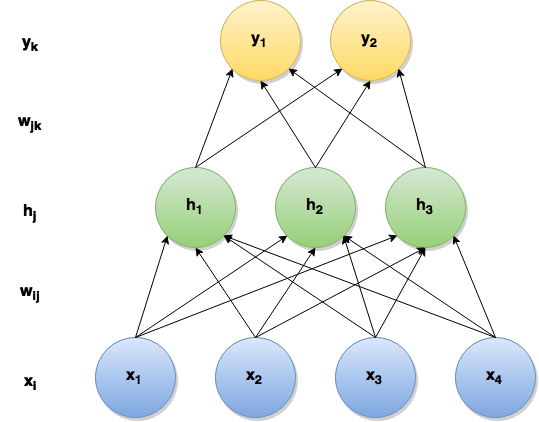
\includegraphics[width=0.9\linewidth]{img/mgr_backprop_net.png}
\end{Figure}

\subsection{Wsteczna propagacja błędów} \label{ssec:backpropagation}
Wsteczna propagacja błędów jest podstawową metodą uczenia nadzorowanego wielowarstwowych jednokierunkowych
sieci neuronowych. Poprzez uczenie nadzorowane należy rozumieć proces uczenia, w~którym sieć neuronowa
otrzymuje dane wraz z~ich etykietami (spodziewanym wyjściem sieci).

W~pierwszym kroku uczenia należy zdefiniować funkcję straty $Loss(w)$ przyjmującą jako~argument wektor wag
sieci neuronowej. Funkcją tą może być średni błąd kwadratowy, dla danych ciągłych:\\
$$Loss(w)=\frac{1}{2}\sum\limits_{m}(\sigma(w^{T}x^{(m)}) - y^{(m)})^2$$
lub entropia krzyżowa, dla danych binarnych:
$$Loss(w)=-\sum\limits_m(\sigma(w^{T}x^{(m)})\log{y^{(m)}} + (1-\sigma(w^{T}x^{(m)})\log{(1-y^{(m)})})
$$
gdzie:
\begin{minipage}[t]{\textwidth}
\begin{itemize}
  \item w - wagi sieci neuronowej,
  \item m - numer próbki uczącej,
  \item x - wartości wejściowe,
  \item y - spodziewane wartości wyjściowe,
  \item $\sigma$ - funkcja aktywacji.
\end{itemize}
\end{minipage}

Celem uczenia sieci jest minimalizacja funkcji $Loss(w)$. Na~początku należy określić gradient funkcji straty
względem wag sieci (gradient jest taki sam dla obu wymienionych powyżej funkcji).
Następnie można przystąpić do~optymalizacji tej~funkcji wykorzystując metodę gradientu prostego.
Kroki tego algorytmu przedstawiono poniżej:
\begin{enumerate}
  \item zainicjuj losowo wektor wag w,
  \item oblicz gradient funkcji straty,
  \item $w:=w-\alpha \nabla Loss(w)$, $\alpha$ - współczynnik określający długość kroku,
  \item wróć do~kroku 2. jeśli nie~został spełniony warunek stopu.
\end{enumerate}

Zakładając, że~wartość błędu dla~danego przykładu uczącego wyraża się~wzorem
$$Error^{(m)}=\sigma(w^{T}x^{(m)})-y^{(m)}$$
gradient funkcji straty ma~wzór:
$$\nabla_{w}Loss=\sum\limits_{m}Error^{(m)}\sigma'(w^{T}x^{(m)})x^{(m)}$$
Ponieważ $\sigma(x)=\frac{1}{1+e^{-x}}$, pochodna funkcji sigmoidalnej wyraża się~wzorem:
$$\sigma'(x)=\sigma(x)(1-\sigma(x))$$

Dla uproszczenia załóżmy, że~w~sieci występuje tylko jedna warstwa ukryta. Wówczas gradient funkcji straty
względem wag połączeń pomiędzy warstwą wyjściową, a~ukrytą:
$$\frac{\partial Loss}{\partial w_{jk}}=\frac{\partial Loss}{\partial in_k}\frac{\partial
in_k}{\partial w_{jk}}= \delta_k \frac{\partial (\sum\limits_j w_{jk}h_j)}{\partial w_{jk}} = \delta_k h_j$$
Poprzez $in_k$ oznaczono wektor wejść trafiających do~funkcji aktywacji poszczególnych neuronów warstwy
wyjściowej.

Gradient funkcjii straty względem wag połączeń pomiędzy warstwą wejściową a~ukrytą:
$$ \frac{\partial Loss}{\partial w_{ij}}=\frac{\partial Loss}{\partial in_j}\frac{\partial in_j}{\partial
w_{ij}} = \delta_j \frac{\partial (\sum\limits_j w_{ij}x_i)}{\partial w_{ij}} = \delta_j x_i $$

$$ \delta_k = \frac{\partial}{\partial in_k}(\sum\limits_k \frac{1}{2}
[\sigma(in_k)-y_k]^2)=[\sigma(\in_k)-y_k]\sigma'(in_k)$$

$$ \delta_j = \sum\limits_k\frac{\partial Loss}{\partial in_k}\frac{\partial in_k}{\partial
in_j}=\sum\limits_k \delta_k \cdot \frac{\partial}{\partial in_j}(\sum\limits_j w_{jk}\sigma(in_j))=[\sum\limits_k \delta_k
w_{jk}]\sigma'(in_j)$$

Jak widać w~ostatnim wzorze: wykorzystujemy gradient obliczony dla~warstwy wyjściowej
do~obliczenia gradientu dla~poprzedniej warstwy. Przy~większej liczbie warstw w~sieci gradienty
dla~kolejnych warstw są~obliczane analogicznie (na~podstawie wartości obliczanych w~następnych warstwach).
Stąd właśnie metoda ta nosi nazwę wstecznej propagacji błędów.


\section{Ogólna koncepcja głębokiego uczenia}
Sama koncepcja głębokiego uczenia nie jest szczególnie nowa. Sieci
wielowarstwowe uczone za pomocą wstecznej propagacji błędów istnieją
już~od~ponad 40 lat. Sieciom tym~towarzyszy jednak poważna wada: przy~wielu
warstwach w~sieci, wagi wyjść początkowych warstw są aktualizowane w~bardzo
nieznacznym stopniu (na ogół: im~większa odległość warstwy od~wyjścia,
tym~mniejsze korekcje wag). W~literaturze problem ten nazywany jest problemem
zanikającego gradientu (\textit{ang. vanishing gradient problem}). Z~tego
powodu do~efektywnego uczenia metodą wstecznej propagacji błędów konieczne jest
stosowanie niewielkiej liczby warstw (w~praktyce stosowano przeważnie
do~czterech warstw). Choć teoretycznie zastosowanie dwóch warstw
wystarcza do~aproksymacji dowolnej funkcji, to~jednak może wymagać bardzo dużej
liczby neuronów w~warstwie ukrytej (w~niektórych problemach liczba neuronów w~warstwie ukrytej może rosnąć
wykładniczo względem rozmiaru danych wejściowych).

Rozwiązaniem problemu zanikającego gradientu jest zastosowanie dodatkowego
etapu: tzw.~uczenia wstępnego (\textit{ang.~pre-training}). W~tym~etapie
optymalizowaną funkcją nie~jest funkcja błędu (jak~w~przypadku metody wstecznej
propagacji błędu), ale~funkcja prawdopodobieństwa wystąpienia danych p(v),
gdzie v stanowi dane wejściowe sieci. Celem, do~którego dąży etap uczenia
wstępnego jest takie uformowanie funkcji p(v), by~dla~danych podobnych do~tych obserwowanych w~zbiorze
uczącym wartość funkcji prawdopodobieństwa była jak największa, natomiast dla pozostałych danych:
jak~najmniejsza.

Opisana metoda uczenia wstępnego zakłada, że~po~kolei uczona jest każda
z~warstw (nie~wszystkie na~raz), zaczynając od~warstwy wejściowej, kończąc
na~wyjściowej. W~jednej iteracji algorytmu uczone są wagi tylko jednej z~warstw.
W~pierwszym kroku algorytmu uczona jest pierwsza warstwa ukryta i~efektem
uczenia powinno być wyodrębnienie takich cech danych, które odróżniają
je~od~danych losowych. W~drugim etapie kolejna warstwa jest uczona w~taki
sposób, by~była w~stanie odróżnić kombinację cech występujących w~danych
od~losowej kombinacji cech itd. Istotną różnicą tej metody w~stosunku do~metody
wstecznej propagacji błędu jest uczenie tylko jednej warstwy na~raz
(po~nauczeniu danej warstwy jej wagi nie~są już modyfikowane w~etapie uczenia
wstępnego). Tak nauczona sieć, choć jeszcze nie~nadaje się~do~przeprowadzania
klasyfikacji, to~dobrze modeluje charakter danych, tzn.~właściwości danych,
które często pojawiają się~w~zestawie uczącym.

\begin{figure}[H]
	\centering
	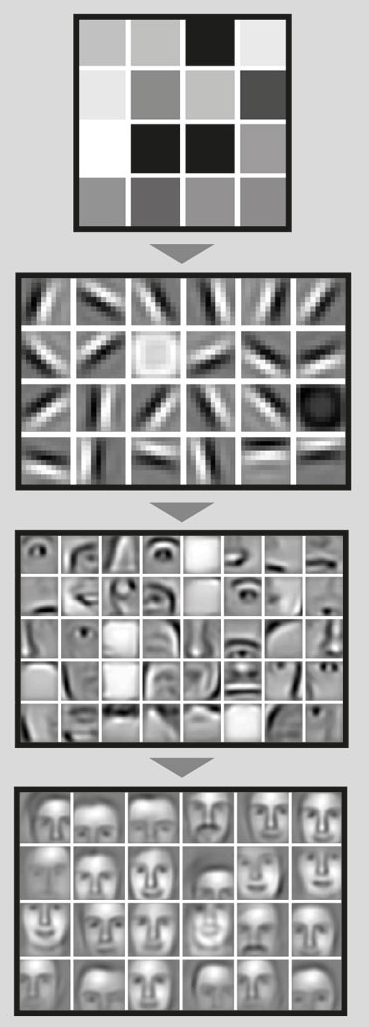
\includegraphics[width=0.45\linewidth]{img/hierarchical-learning_cropped.jpg}
	\caption{cs.stanford.edu}
\end{figure}

Po~etapie uczenia wstępnego następuje tzw. dostrajanie sieci
(\textit{ang.~fine-tuning}). W~tym etapie dodawana jest warstwa wyjściowa sieci.
Następnie cała sieć jest uczona danymi etykietowanymi (uczenie nadzorowane)
metodą wstecznej propagacji błędu. Dzięki zastosowaniu uczenia wstępnego
sztuczna sieć neuronowa znacznie lepiej generalizuje funkcję, którą ma~modelować
(tzn.~jest znacznie mniej podatna na~tzw.~overfitting, czyli zbytnie dopasowanie modelu do~danych).
Ponadto, do~dostrajania jest potrzebna znacznie mniejsza ilość danych niż do~pierwszego etapu. Zatem
do~uczenia sieci wystarczy, by~tylko niewielka część danych uczących była
etykietowana.

\section{Modelowanie funkcji prawdopodobieństwa}
Cechą wspólną wszystkich mechanizmów głębokiego uczenia badanych w~ramach tej~pracy magisterskiej jest
wykorzystanie etapu uczenia wstępnego, którego celem jest odpowiednie zamodelowanie
funkcji rozkładu prawdopodobieństwa, tzn.~osiągnięcie takiego rozkładu prawdopodobieństwa p(v),
że~danym~wejściowym v, które są podobne do~danych uczących, będą odpowiadały wysokie wartości
funkcji prawdopodobieństwa, natomiast pozostałym danym (w~szczególności danym losowym) będzie odpowiadało
niskie prawdopodobieństwo.

Do modelowania funkcji prawdopodobieństwa można wykorzystać wiele mechanizmów. W~tej~pracy omówiona zostanie
jedynie \textbf{Ograniczona Maszyna Boltzmanna} (\textit{ang.~Restricted Boltzmann Machine}).

\subsection{Autoenkoder}
Autoenkoder \cite{Autoencoder} to~sieć neuronowa, która składa się z~trzech warstw:
\begin{itemize}
	\item warstwy wejściowej,
	\item warstwy ukrytej,
	\item warstwy wyjściowej.
\end{itemize}

\begin{figure}[H]
	\centering
	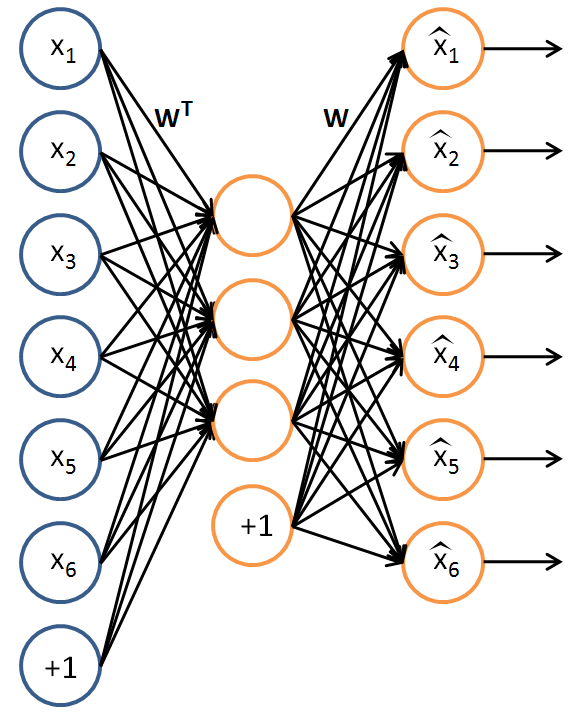
\includegraphics[width=0.75\linewidth]{img/autoencoder.png}
	\caption{Autoenkoder}
\end{figure}

Dodatkowo liczba neuronów w~warstwie wyjściowej jest równa liczbie neuronów w~warstwie wejściowej.
Celem uczenia takiej sieci jest osiągnięcie stanu, w~którym wartości na~wyjściu sieci są równe
wartościom wejściowym tej sieci. Wówczas sieć ma za zadanie wykształcenie przekształcenia tożsamościowego.

\subsubsection{Zastosowania}
Zazwyczaj w~warstwie ukrytej takiej sieci umieszcza się~mniej neuronów niż~w~dwóch pozostałych warstwach.
Neurony tej warstwy w~procesie uczenia zaczynają wykrywać różne często pojawiające się powiązania
wśród wartości wejściowych (np.~mogą zauważyć, że gdy pierwsza z~wartości jest równa jeden,
wówczas trzecia i czwarta są równe zero itp.).
Pozwala to~na~kompresję danych.

Innym zastosowaniem mechanizmu autoenkodera jest korekcja danych. Wówczas w~warstwie ukrytej
może być więcej neuronów niż w~warstwie wejściowej/wyjściowej. Tak nauczona sieć, po~otrzymaniu na~wejściu
wektora wejściowego zawierającego pewne błędy w~danych (np.~szumy), potrafi dokonać korekty danych,
a dane poprawione pojawią się~na~wyjściu sieci.

W~ogólności warstwa wejściowa oraz warstwa ukryta autoenkodera tworzą razem mechanizm kodujący, a~warstwa ukryta wraz
z~warstwą wyjściową tworzą mechanizm dekodujący.

\subsubsection{Funkcja kosztu}
Dla danych ciągłych ($x\in\mathbb{R}$) jako funkcję kosztu typowo stosuję się średni kwadrat błędu:
\begin{equation*}
\frac{1}{2N}\sum\limits_{i=1}^{s_1}(x-\hat{x})^2
\end{equation*}
gdzie $N$ to~liczba klasyfikowanych przykładów, $s_1$ to~długość wektora wejściowego (jak~również wyjściowego),
$x$ to~wektor wartości wejściowych, a~$\hat{x}$ to~wektor wartości wyjściowych. Suma dzielona jest przez $2N$ zamiast
$N$ w~celu~wygodniejszego liczenia pochodnej w~procesie uczenia. Zabieg ten ma charakter czysto estetyczny.

\subsubsection{Regularyzacja rozrzutu}
W~autoenkoderze staramy się~zapewnić, by~średnia wartość na~wyjściu każdego neuronu warstwy ukrytej
(średnia liczona po~przykładach trenujących) była bliska pewnej z~góry przyjętej wartości zwanej \textbf{parametrem
rozrzutu} (\textit{ang.~sparsity parameter})). Zwykle parametr ten przyjmuje niewielkie wartości (np. 0,05). Dzięki temu
dla~większości danych wejściowych niewiele neuronów warstwy ukrytej będzie ,,aktywowanych'', a~więc każdy neuron będzie
rozpoznawał jedną wybraną zależność pomiędzy danymi i~będzie stwierdzał czy~w~danym wektorze wejściowym jest ona obecna
(wartość na~wyjściu neuronu równa 1) czy też nie (wartość na~wyjściu neuronu równa 0). W~celu osiągnięcia odpowiedniego
rozrzutu funkcja celu musi przyjmować odpowienio wyższe wartości, gdy wartość średnia dla wzbudenia neuronu warstwy
ukrytej jest różna od~zadanego parametru rozrzutu. Założony cel można osiągnąć poprzez zastosowanie funkcji kosztu
w~postaci dyvergencji Kullbacka-Leiblera:
\begin{equation*}
\sum\limits_{j=1}^{s_2}KL(\rho||\hat{\rho_j}) = \sum\limits_{j=1}^{s_2}\rho \log\frac{\rho}{\hat{\rho_j}} +
(1-\rho)\log\frac{1-\rho}{1-\hat{\rho_j}}
\end{equation*}
gdzie $s_2$ to~liczba neuronów w~warstwie ukrytej, j to~numer neuronu w~warstwie ukrytej, $\rho$~to~parametr rozrzutu,
a~$\hat{\rho_j}$ to~średnia wartość na~wyjściu j-tego neuronu wartstwy ukrytej.

Po~uwzględnieniu regularyzacji, funkcja kosztu przyjmie postać:
\begin{equation*}
J(W,b)=\frac{1}{N}\sum\limits_{i=1}^{s_1}(x-\hat{x})^2 + \beta\sum\limits_{j=1}^{s_2}KL(\rho||\hat{\rho_j})
\end{equation*}
gdzie $W$ i $b$, to~odpowiednio wagi sieci i~bias.

\subsubsection{Uczenie}
Do~uczenia sieci wykorzystywana jest metoda wstecznej propagacji błędów (opisana we~wcześniejszej części pracy),
stąd proces zmiany wag w~sieci zaczyna się~od~warstwy wyjściowej. Zdefiniujmy różnicę pomiędzy wartościami wyjściowymi
a wejściowymi jako $\delta_i^{(3)}$, gdzie $i$ jest numerem neuronu w~warstwie wyjściowej.
Wagi warstwy wyjściowej aktualizujemy wg wzoru \ref{eqn:wagi_autenc}:
\begin{equation}
    \begin{split}
    W'_i &= W_i + \alpha\delta^{(2)}_i \\
    \delta_i^{(2)} &= \left( \left( \sum\limits_{j=1}^{s_{2}} W^{(2)}_{ji} \delta^{(3)}_j \right)
    + \beta \left( - \frac{\rho}{\hat\rho_i} + \frac{1-\rho}{1-\hat\rho_i} \right) \right) f'(z^{(2)}_i)
    \end{split}
    \label{eqn:wagi_autenc}
\end{equation}
gdzie $f'$ to~pochodna funkcji aktywacji używanej w~neuronach, a~$z^{(2)}_i$, to~wartości preaktywacji neuronów warstwy
ukrytej (wartości, które trafiają do~funkcji aktywacji tych neuronów).

Wagi wastwy ukrytej odpowiadają transponowanej macierzy wag warstwy wyjściowej. Jest tak~dlatego, że~jak~wcześniej
wspomniano, warstwa wyjściowa odpowiada za~operację odwrotną do~operacji wykonywanej przez~warstwę ukrytą (odpowiednio:
dekodowanie i kodowanie).

\subsection{Ograniczona Maszyna Boltzmanna}
Ograniczona Maszyna Boltzmanna jest sztuczną siecią neuronową składającą się~z~dwóch warstw neuronów:
\begin{itemize}
  \item warstwy neuronów wejściowych,
  \item warstwy neuronow ukrytych.
\end{itemize}

\begin{figure}
	\centering
	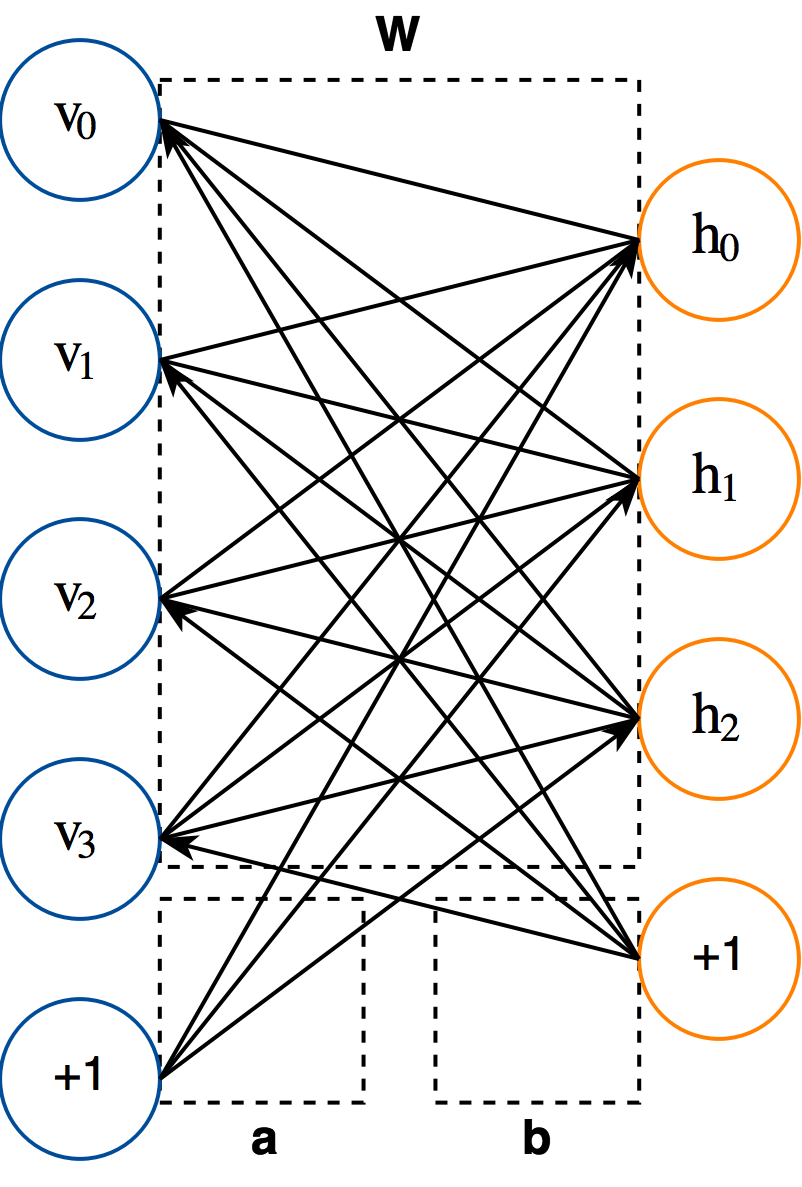
\includegraphics[width=0.75\linewidth]{img/RBM.png}
	\caption{Ograniczona Maszyna Boltzmanna}
\end{figure}

Cechą charakterystyczną tego mechanizmu jest jego umiejętność do~odszukiwania cech danych wejściowych
(\textit{ang. feature extraction}). Przykładowo Ograniczona Maszyna Boltzmanna, którą uczono obrazkami, będzie
wykrywać charakterystyczne łuki czy krawędzie.

Dzięki tej właściwości mechanizm może być wykorzystywany m.in. do~korekcji danych czy~wręcz do~ich~generowania
(np.~do~generowania pisma ręcznego).

\subsubsection{Prawdopodobieństwo stanów sieci}
W~Ograniczonej Maszynie Boltzmanna każdy stan sieci (tzn. zestaw wartości wyjść poszczególnych neuronów)
ma~określone prawdopodobieństwo zadane wzorem:

$p(v,h)=\frac{1}{Z}e^{-E(v,h)}$, gdzie:
\begin{itemize}
  \item v to~macierz wyjść neuronów wejściowych,
  \item h to~macierz wyjść neuronów ukrytych,
  \item Z to~czynnik normalizujący (tzw.~funkcja partycji),
  \item $E(v,h)=-a^{T}v-b^{T}h-v^{T}Wh$,
  \item a,b oraz W to~macierze wag sieci.
\end{itemize}

\subsubsection{Inferencja}
Ze~względu na~to, że~neurony nie~łączą się~ze~sobą w~obrębie tej~samej warstwy, wartość na~wyjściu każdego
neuronu w~danej warstwie można uzyskać wyłącznie na~podstawie wartości wyjść neuronów drugiej warstwy.
Prawdopodobieństwa wzbudzeń neuronów można efektywnie obliczyć korzystając z~wzorów:
\begin{equation}
    \begin{split}
        p(h_{j}=1|v)&=\sigma(b_{j}+\sum\limits_{i=1}^{m}w_{i,j}v_{i}) \\
        p(v_{i}=1|h)&=\sigma(a_{i}+\sum\limits_{j=1}^{n}w_{i,j}h_{j})
    \end{split}
	\label{eqn:rbm_inference}
\end{equation}
gdzie: $\sigma$ to~funkcja aktywacji, $i$ oraz $j$ to~numery kolejnych neuronów (odpowiednio: wejściowych i~ukrytych).


\subsubsection{Uczenie}
Celem uczenia sieci jest znalezienie takich parametrów a,b i W, że~wartość funkcji prawdopodobieństwa p(v)
dla~danych obserwowanych będzie wysoka, a~dla~pozostałych danych niska. W~praktyce zamiast maksymalizować
funkcję prawdopodobieństwa p(v), minimalizuje się funkcję średniego ujemnego log-prawdopodobieństwa:
$$\frac{1}{T}\sum\limits_{t}-\log{p(v^{(t)})}$$

Do~minimalizacji funkcji metodami gradientowymi konieczne jest obliczenie pochodnej po~parametrach sieci
dla tej funkcji:
$$\frac{\partial-\log{p(v^{(t)})}}{\partial{\theta}}=\mathbb{E}_h[\frac{\partial{E(v^{(t)},h)}}{\partial{\theta}}\mid{v^{(t)}}]-\mathbb{E}_{v,h}[\frac{\partial{E(v,h)}}{\partial{\theta}}]$$

Pierwszy ze~składników sumy występującej w~powyższym wzorze to~tzw. składnik pozytywny. Drugi składnik
to~tzw.~składnik negatywny. Pierwszy z~nich odpowiada zwiększaniu wartości funkcji prawdopodobieństwa
dla~obserwowanych danych, a~drugi zmniejsza prawdopodobieństwo danych nieobserwowanych. Drugi składnik jest
skomplikowany obliczeniowo, gdyż występuje w~nim iteracja po~wszystkich możliwych stanach sieci, których
liczba rośnie wykładniczo względem liczby neuronów w~sieci. Z~tego powodu dokonuje się estymacji. Jedną
z~wykorzystywanych metod jest tzw. próbkowanie Gibbsa. 

\textbf{Próbkowanie Gibbsa} pozwala wyeliminować problem obliczania wartości oczekiwanej dla~wszystkich
możliwych stanów sieci. Zamiast tego wartość ta~jest estymowana za~pomocą algorytmu, którego kroki
przedstawiono poniżej.

Próbkowanie Gibbsa (algorytm):
\begin{enumerate}
  \item Oblicz wartości wyjściowe dla~każdego neuronu z~warstwy ukrytej na~podstawie danych wejściowych
  (korzystając z~wzorów \ref{eqn:rbm_inference}).
  \item Oblicz wartości wyjściowe dla~każdego neuronu z~warstwy wejściowej na~podstawie obliczonych wartości
  wyjściowych neuronów ukrytych (korzystając z~wzorów \ref{eqn:rbm_inference}).
\end{enumerate}

Kroki 1 i 2 mogą być powtarzane wielokrotnie, choć w~praktyce okazuje się, że wystarczy jeden
przebieg algorytmu. Otrzymane w~punkcie drugim ,,odtworzone'' wartości wejścia oznaczane są~jako $\tilde{v}$.

\paragraph{Aktualizacja parametrów sieci}
Parametry (wagi) sieci aktualizowane są według następujących wzorów:
\begin{itemize}
  \item $W_t=W_{t-1}+\alpha(h(v^{(t)})v^{(t)T}-h(\tilde{v})\tilde{v}^{T})$
  \item $b_t=b_{t-1}+\alpha(h(v^{(t)})-h(\tilde{v}))$
  \item $a_t=a_{t-1}+\alpha(v^{(t)})-\tilde{v})$
\end{itemize}
\vspace{1cm}

Przez $h(v)$ oznaczono wartości wyjściowe neuronów ukrytych obliczone na~podstawie wartości wyjściowych
neuronów wejściowych.
